\chapter{OpenMOLE \& GridScale} \label{DesignChapter}

The first part of this chapter expands on the goals, features, architecture and components of the open-source OpenMOLE project. We also explore use cases of the system by looking at a simple workflow. The second part of the chapter describes the structure and design of GridScale, the library OpenMOLE relies on to leverage distributed computing resources from grids and clusters.

\section{OpenMOLE}

OpenMOLE\cite{OpenMOLE} is a workflow execution engine that focuses both on allowing expressive definitions of data processing pipelines and delegation of those tasks to remote execution environments \cite{Leclaire2016}. Compared to other existing workflow management systems like Kepler \cite{Kepler}, Taverna \cite{Taverna}, Galaxy \cite{Galaxy} or Pegasus \cite{Pegasus}, it does not target a specific scientific community and instead aims at offering formalisms that can be used to create generic pipelines.

One of the main objectives of OpenMOLE is embedding workflow models and definitions provided by users in many different forms \cite{Reuillon2013}. Generally, other workflow engines have rigid, text-based rules used to describe individual tasks and their connections, while providing limited support for calling external programs. 

However, OpenMOLE uses a DSL\footnote{Domain Specific Language} built on top of Scala\cite{Scala} to embed a wide variety of tasks defined in any programming language based on the Java Virtual Machine (Java, Scala, Clojure, Groovy, Kotlin). Additionally, prepackaged binaries, C++ executables and Python scripts that depend on shared libraries or pre-loaded packages are seamlessly integrated into workflows. Benefits of relying on Scala's type system include more meaningful task descriptions and early error detection since potential mistakes are caught at compile-time, instead of only after submission to grids or clusters.

Possible execution environments include the user's local machine, SSH servers, grids or self-hosted clusters operated by one of the many supported schedulers: SGE \cite{SGE}, SLURM, PBS \cite{PBS}, HTCondor \cite{HTCondor}, OAR \cite{OAR} or Torque \cite{Torque}. These are all enabled by GridScale \cite{Reuillon2016}, the self-contained library that is shipped by default with OpenMOLE and handles job management on distributed computing environments.

The OpenMOLE platform is now mature and has engaged a loyal user base. It is regularly used for large scale experiments and its robustness in combination with GridScale was proven by experiments where it has been used to run half a billion tasks on EGI\footnote{European Grid Initiative} \cite{Schmitt2015}.

\subsection{Architecture}

The design of the application has been guided by the total decoupling between the creation of the pipelines describing the scientific algorithms and their execution on remote environments \cite{Leclaire2016}. As shown in Figure \ref{OpenMOLEArch}, this led to a layered structure, where the actual experiments are independent from how the tasks they incorporate are run and managed or how the resource requirements are serviced.

\begin{figure}[h]
	\centering
		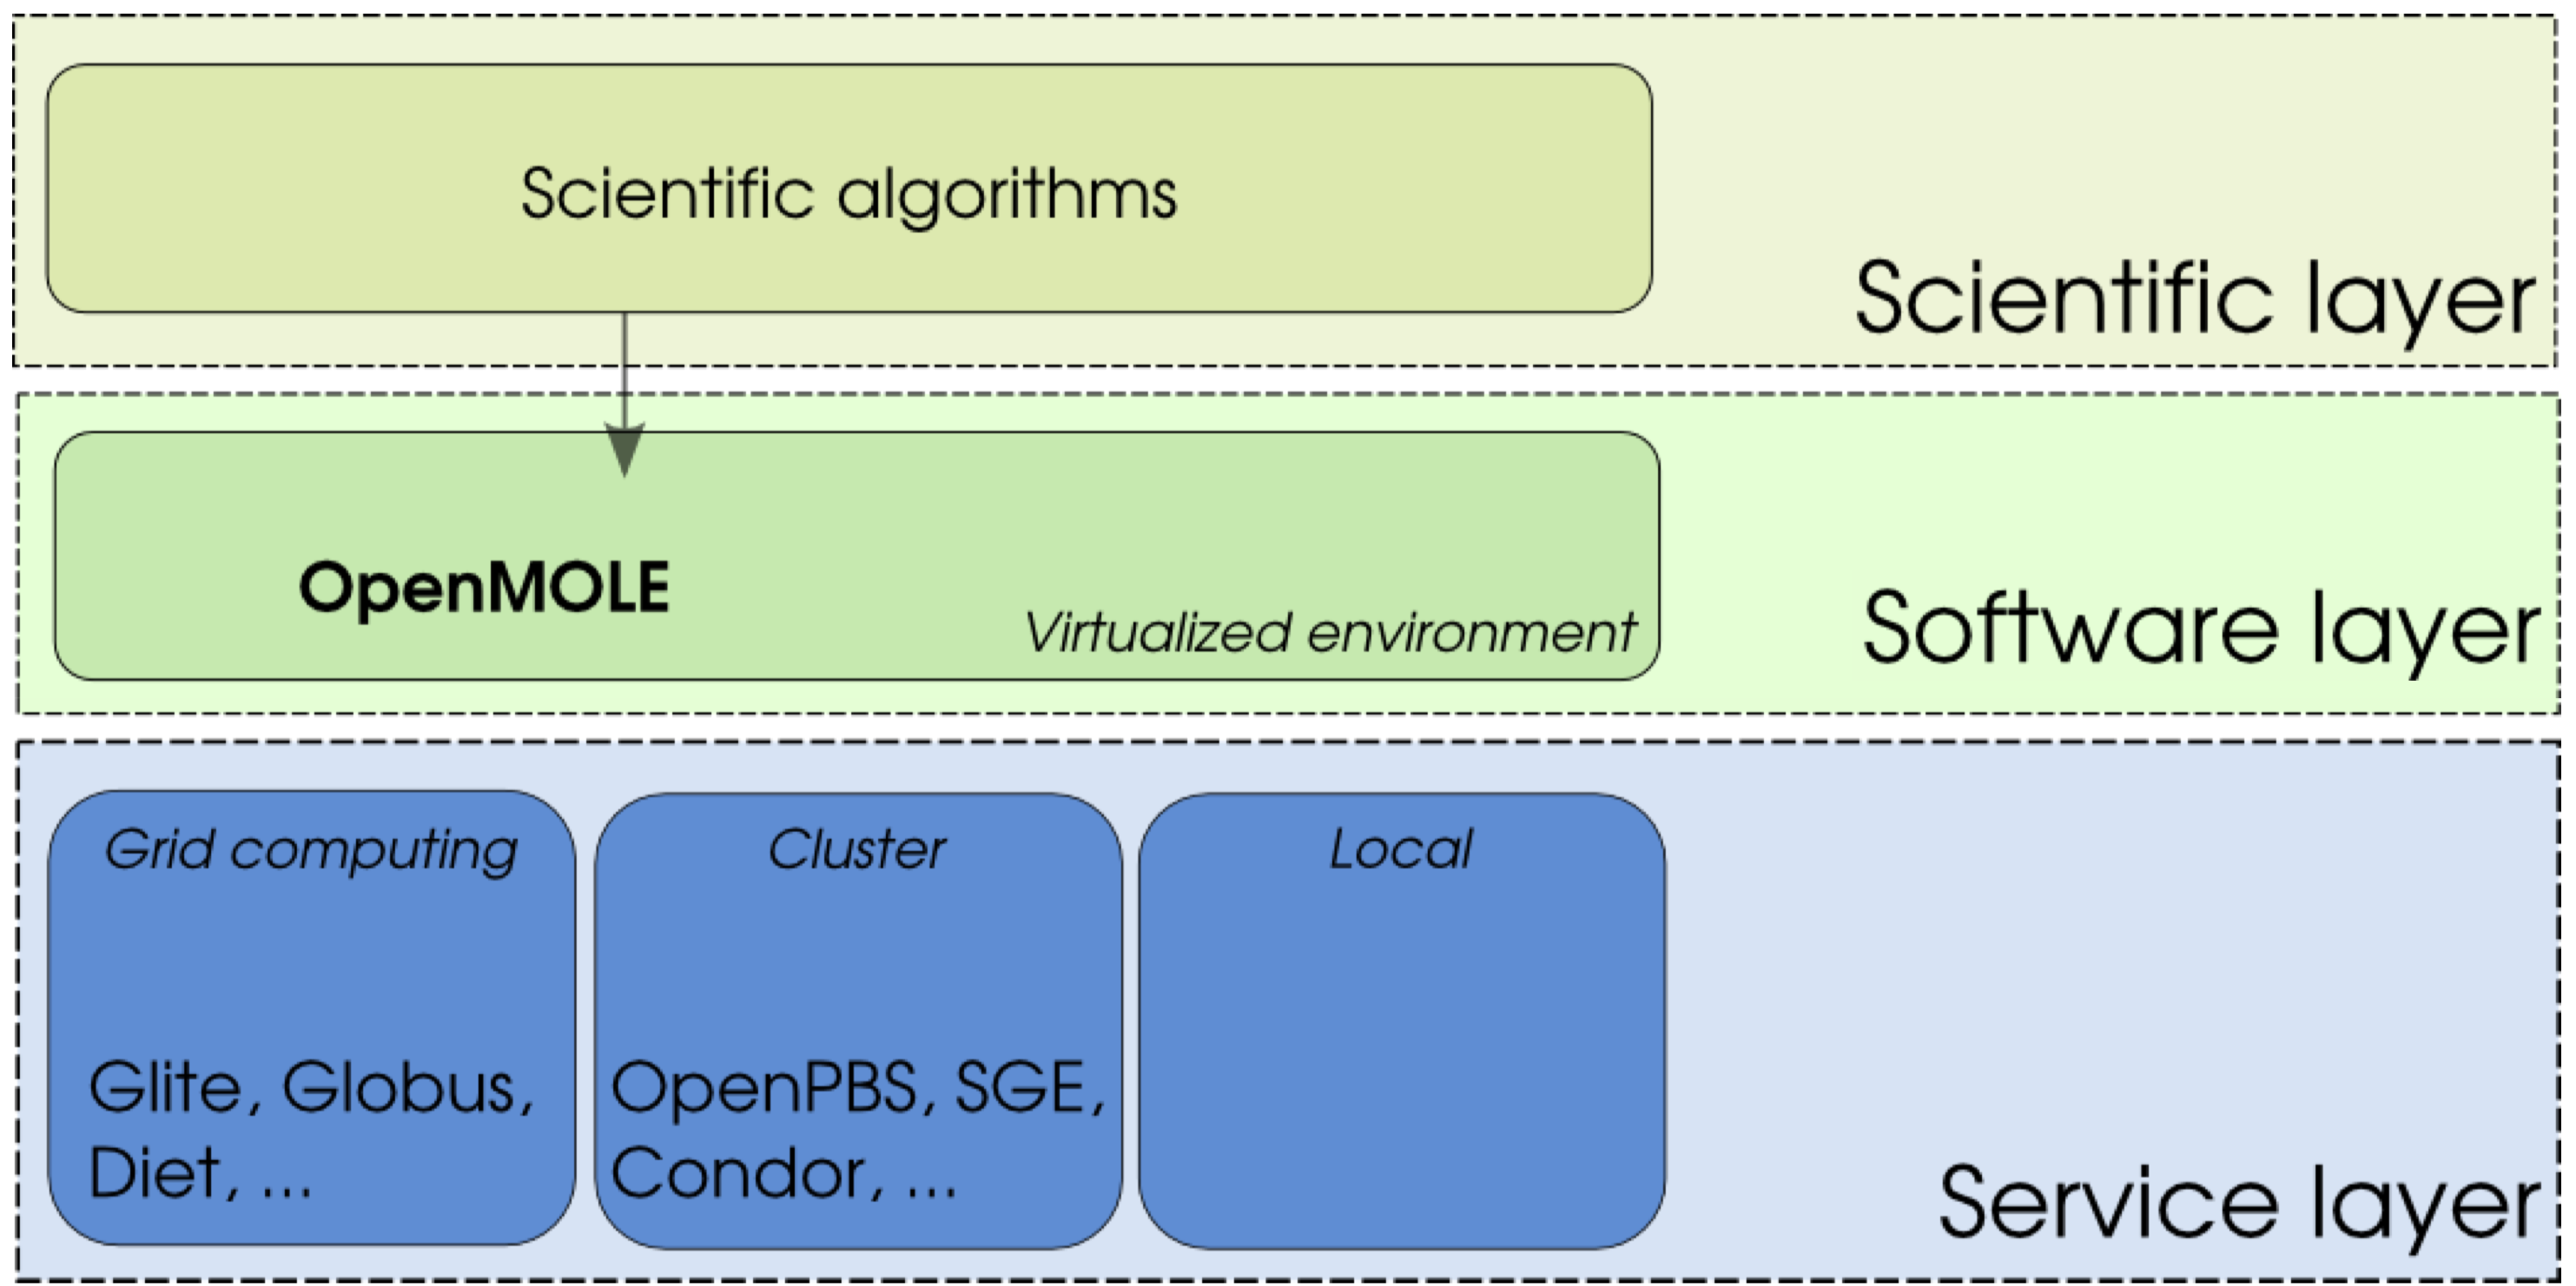
\includegraphics[width=0.9\linewidth]{OpenMOLEArch.png}
	\caption{OpenMOLE layered architecture \cite{Reuillon2010}.}
	\label{OpenMOLEArch}
\end{figure}

In this context, the user is not concerned with how the execution environment is provisioned and can change it easily without altering the workflow description. Additionally, this allows for a fine granularity of task distribution since individual tasks can be sent to environments tailored specifically for their requirements. A clear use case for this are jobs that need to be accelerated using GPUs, with other parts of the workflow running on CPUs as usual.

The structural layers fulfil completely different roles and are modular blocks with clearly defined roles:
\begin{itemize}
	\item The scientific layer relies on the DSL. It is where the user defines the workflow and specifies data sources and execution environments.
	\item The software layer is concerned with the translation of the workflow specification to an internal representation consisting of runnable jobs and their dependencies. It uses the Scala actor model \cite{ScalaActors} to coordinate the whole process of installing the OpenMOLE runtime on each remote execution site, continuously monitoring the status of outstanding jobs, or feeding results of completed tasks to the subsequent ones using them as input. New remote environments are simply added as plugins and they are essentially adapters to the resources exposed by the service layer.
	\item The GridScale library is the service layer, presented in Section \ref{GridScaleSection}.
\end{itemize}

\subsection{Domain Specific Language}

\textit{Tasks} are the basic construct of workflows in OpenMOLE. They essentially consist of a computation that is run against a set of \textit{inputs} to produce a set of \textit{outputs}. Together with \textit{transitions}, which transfer outputs of individual tasks to inputs of subsequent ones, they establish the simplest form of data pipeline.

Listing \ref{SimpleWorkflow} shows a very basic workflow that computes the square of each number from 1 to 100. It begins by declaring variables \verb|i| and \verb|res|, which represent the dataflow and are used to carry results between tasks that are connected via transitions. Since the DSL is build as a set of extensions on top of the Scala programming language, the variables are statically typed, which enables formal verification of the workflow at compile time \cite{Reuillon2013}. This ensures that runtime type mismatches of data transmitted between tasks cannot occur.

\begin{listing}[h]
	\centering
	\begin{minipage}{10.6cm}
		\begin{minted}[frame=single,framesep=2mm,baselinestretch=1.15,fontsize=\small,linenos]{scala}
val i = Val[Int]
val res = Val[Int]

val exploration = ExplorationTask(i in (1 to 100 by 1))

val model =
  ScalaTask("val res = i * i") set (
    inputs += i,
    outputs += (i, res)
  )

val env = LocalEnvironment(8)

exploration -< (model on env hook ToStringHook())
		\end{minted}
	\end{minipage}
	\caption{Simple OpenMOLE workflow.}
	\label{SimpleWorkflow}
\end{listing}

Lines 6-10 define the actual model that we want to compute. In this case, the specification is a \verb|ScalaTask|, where for each input of type \verb|i| the output is a tuple \verb|(i, res)|. Concretely, for input \verb|5|, the output will be \verb|(5, 25)|. Apart from Scala code, a \verb|ScalaTask| can embed code from any programming language running on the JVM (Java, Clojure, Groovy). Other types of tasks include \verb|MoleTask|, used to embed entire predefined workflows, or \verb|CARETask|, used to run any type of prepackaged binary and discussed in section \ref{CARESection}.

One of the central objectives of OpenMOLE is to allow parameter optimisation for the models it executes. The sampling of parameters is achieved through the use of \textit{explorations} in the language. Every parameter sampled from a set is combined with all the other parameters to generate the workflow input. In our case, the exploration at line 4 only samples parameter \verb|i|, so the model will be replicated 100 times and executed with an integer between 1 and 100 as input.

Line 12 instantiates the environment where the workflow will be run. Here we select a \verb|LocalEnvironment| and allow the computation to create and use 8 threads on the local machine. Line 14 ties all the building blocks together. The exploration generates all possible values of \verb|i| and the model is executed on the given environment for each one of them. The \verb|-<| symbol represents a divergent transition between the exploration and the task, each output of the sampling being fed to the model.

In OpenMOLE, \textit{hooks} are used to extract the results of running an experiment. They are executed every time the task that they are assigned to terminates and can perform actions like simply displaying the data or saving it to CSV\footnote{Comma-separated values} files. Here the \verb|ToStringHook| simply prints the output of each task.

Figure \ref{OpenMOLEWorkflow} shows a graphical representation of the combination of primitives described above. This is how a workflow is designed using the graphical user interface instead of the specification language.

\begin{figure}[h]
	\centering
		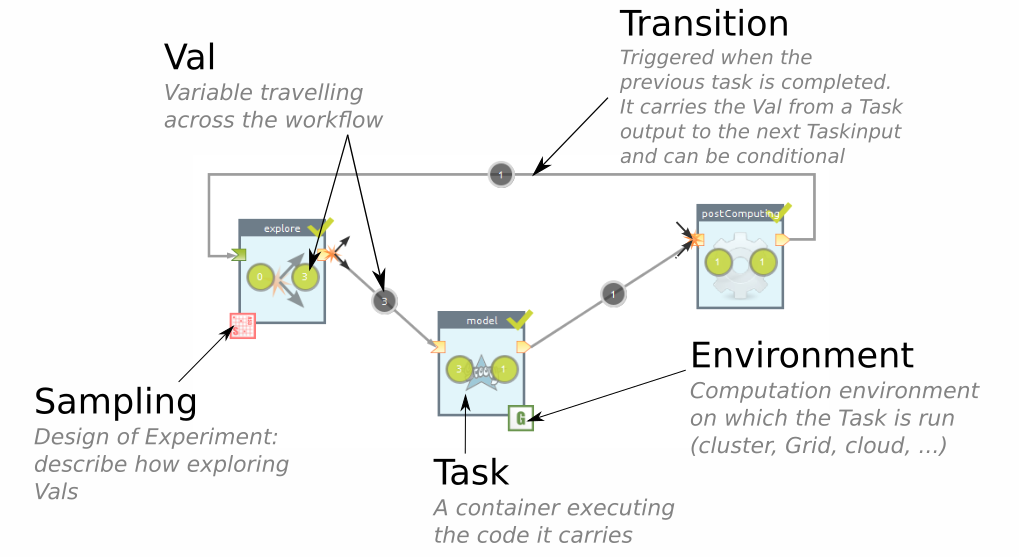
\includegraphics[width=0.8\linewidth]{OpenMOLEWorkflow.png}
	\caption{OpenMOLE workflow \cite{OpenMOLE}.}
	\label{OpenMOLEWorkflow}
\end{figure}

Going beyond the simple example, Listing \ref{Sampling} shows a sampling that explores all combinations of a discrete parameter \verb|i|, a continuous parameter \verb|j|, a file \verb|f| from the given \verb|workDirectory| and a random seed \verb|s| sampled from a uniform distribution. This is achieved using the \textit{x} combinator, which unrolls the domain for each parameter before combining all the possibilities \cite{OpenMOLEDSL}.

\todo[inline]{It's basically a cartesian product of the parameter sets}


\begin{listing}[h]
	\centering
	\begin{minipage}{10.6cm}
		\begin{minted}[frame=single,framesep=2mm,baselinestretch=1.15,fontsize=\small,linenos]{scala}
val i = Val[Int]
val j = Val[Double]
val f = Val[File]
val s = Val[Long]

val exploration = 
  ExplorationTask(
	(i in (0 to 10)) x 
	(j in (0.0 to 100.0 by 10.0)) x
	(f in (workDirectory / "inputs")) x 
	(s in (UniformDistribution[Long]() take 10))
  )
		\end{minted}
	\end{minipage}
	\caption{Advanced exploration \cite{Leclaire2016}.}
	\label{Sampling}
\end{listing}

Listing \ref{Transitions} shows different transitions that can be used to combined task. Note that, for brevity, we did not include any hooks that would collect the results at any stage. 

The execution on line 13 explores the parameter space and feeds each possible value sequentially through each of the 3 tasks. On line 14, \verb|t2| and \verb|t3| are run in parallel on the inputs received from \verb|t1|. Line 15 demonstrates a convergent transition, where the \verb|>-| operator is used to allow an aggregation task to collect and process the results of the run.

\begin{listing}[h]
	\centering
	\begin{minipage}{12.4cm}
		\begin{minted}[frame=single,framesep=2mm,baselinestretch=1.15,fontsize=\small,linenos]{scala}
val i = Val[Int]

val t1 = ScalaTask("i = i * 2") set ( inputs += i, outputs += i )
val t2 = ScalaTask("i = i * 3") set ( inputs += i, outputs += i )
val t3 = ScalaTask("i = i * 4") set ( inputs += i, outputs += i )

val exploration = ExplorationTask( i in (0 to 100) )
val aggregate = ScalaTask("val i = input.i.sum") set (
  inputs  += i.toArray,
  outputs += i
)

exploration -< t1 -- t2 -- t3
exploration -< t1 -- (t2, t3)
exploration -< t1 -- t2 -- t3 >- aggregate
		\end{minted}
	\end{minipage}
	\caption{Transition types \cite{OpenMOLEDSL}.}
	\label{Transitions}
\end{listing}

Our initial example showed the simple case of running a workflow on the user's machine using a \verb|LocalEnvironment|. However, this is only usually done for testing locally before scaling the experiment and other types of environments are used for real experiments. Listing \ref{Environments} shows examples of instantiating SSH servers and cluster environments.

The user can be authenticated either with a login and password combination, or via a private key. Here we define the authentication by specifying the path to the private key, the associated login and the remote machine's full address. The \verb|encrypted| parameter references a function that will prompt the user for the key's password in case it is protected.

Environments are created by providing the shell login on the remote machine and its address. For the SSH server, we also specify the number of cores that can be used by the workflow. Cluster environments require that the target machine can act as the master of the cluster, being able to take commands for submitting and querying job status.

\begin{listing}[h]
	\centering
	\begin{minipage}{11.5cm}
		\begin{minted}[frame=single,framesep=2mm,baselinestretch=1.15,fontsize=\small,linenos]{scala}
SSHAuthentication += 
  PrivateKey(
    "path/to/private/key",
    "login",
    encrypted, 
    "machine-address")

val sshEnv = SSHEnvironment("login", "machine-address", 8)
val condorEnv = CondorEnvironment("login", "master-address")
val sgeEnv = SGEEnvironment("login", "master-address")
		\end{minted}
	\end{minipage}
	\caption{Usage of various environments.}
	\label{Environments}
\end{listing}

The aim is to provide a similar \verb|AWSEnvironment| primitive, which only receives the user's AWS credentials as parameters. This should automatically create a cluster backed up by EC2 instances and configure it with a scheduler that distributes job submissions generated by the workflow.


\todo[inline]{You need to highlight that even more as it's the take home message for this section: "here is litterally what we want to do!"}

\subsection{Job Distribution}

Compared to other workflow platforms, OpenMOLE follows a zero-deployment approach, meaning that it does not rely on any software being installed on the target machines that the task-generated jobs will run on \cite{Reuillon2013}. In order to support this, a setup phase is required before the task execution step itself. This involves uploading several components to the remove environment \cite{Reuillon2010}:

\begin{itemize}
	\item The OpenMOLE runtime, which includes the OpenMOLE framework and the Java Virtual Machine used to run it.
	\item Task descriptions along with their serialized execution contexts, which describe variables used by the task to transport data.
	\item Resource files used by the tasks.
\end{itemize}

After all the dependencies are in place, a job is packaged to reference the runtime, task and context it corresponds to. Once it is assigned to an execution node by the environment's native submission system, it downloads the runtime and runs the task in the given context. Note that the potentially expensive step of copying the runtime on each node is rarely necessary in practice, since clusters and grids usually operate on filesystems shared across all nodes. OpenMOLE also maintains a cache of the file replicas already uploaded to remote storages, so that a file never gets uploaded twice to the same storage as long as it's not been modified on the host system.

Once finished, jobs upload their results to the storage system. Meanwhile, the OpenMOLE framework continuously tracks the state of the job by querying the submission system and downloads the outputs on the local machine of the user upon completion. The whole process is presented as a sequence diagram in Figure \ref{OpenMOLERuntime}.

\begin{figure}[H]
	\centering
		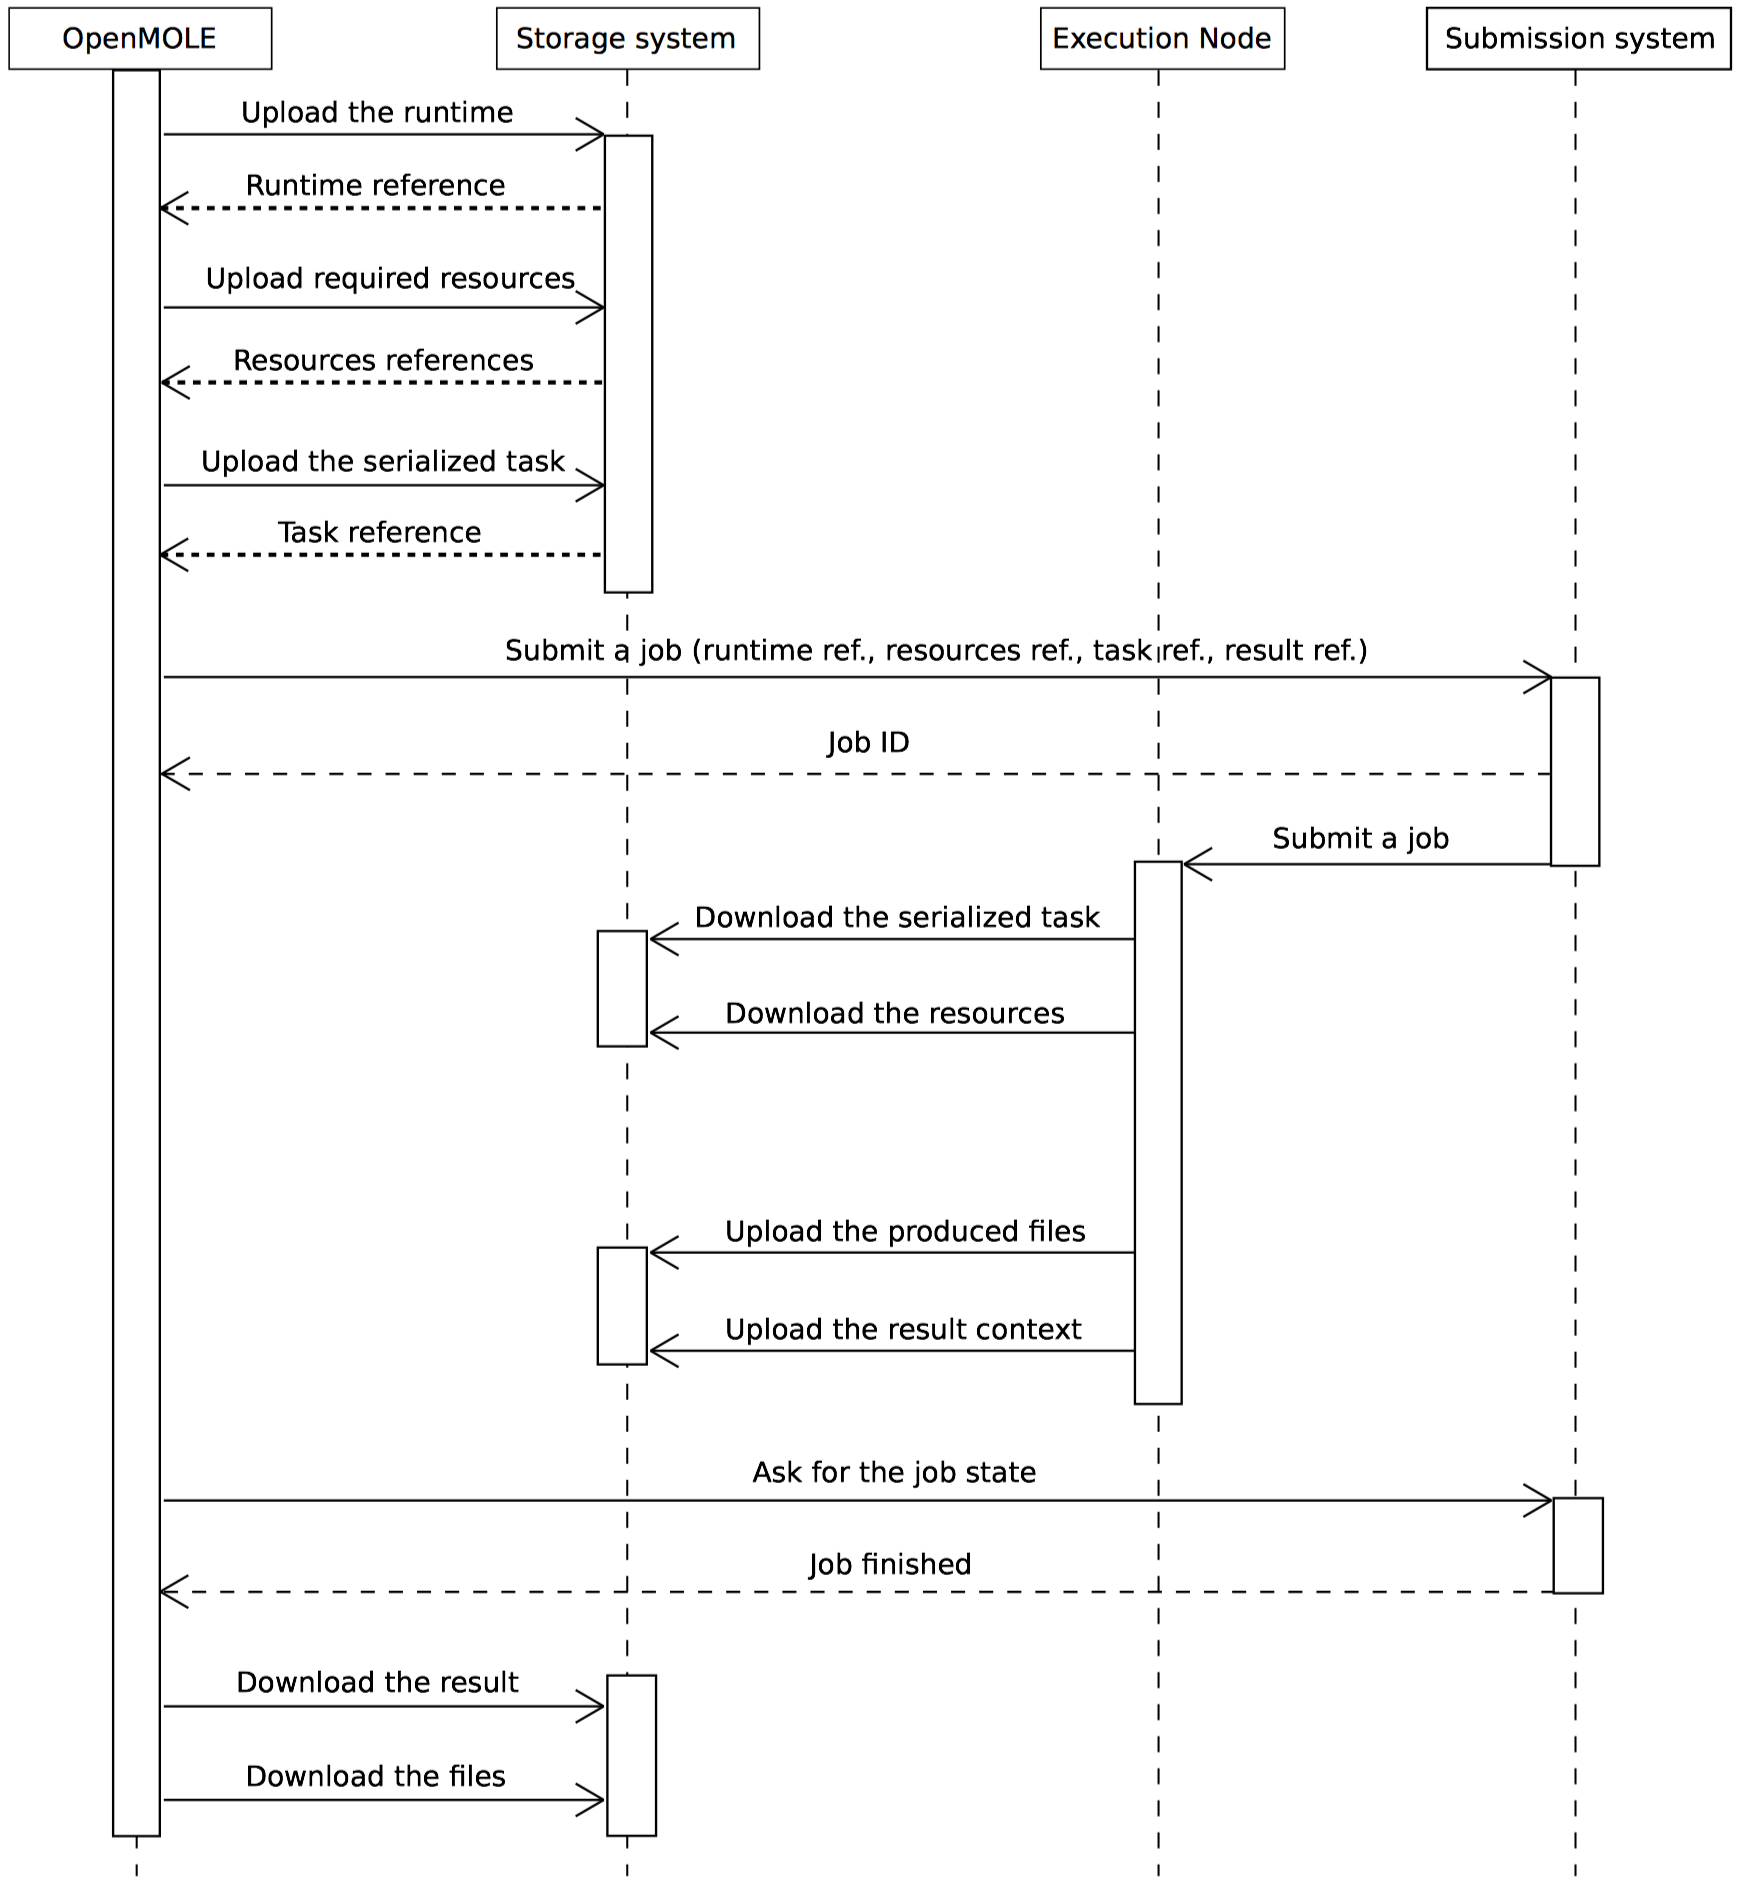
\includegraphics[width=1\linewidth]{OpenMOLERuntime.png}
	\caption{Delegation of a task to remote execution environment in OpenMOLE. \cite{Reuillon2010}.}
	\label{OpenMOLERuntime}
\end{figure}

\subsection{CARE} \label{CARESection}

Resolution of dependencies is a classical problem in the context of job distribution to remote environments, especially in the case of having little to no control over their configuration. Compiled binaries like C++ applications require shared libraries at runtime, while interpreted languages depend on various packages to be present on the execution node. 

Users of grids and clusters do not usually have access to install the needed dependencies. Grids are particularly tricky, since they represent shared pools of heterogeneous resources that are likely to be configured and deployed differently than on a local machine that a workflow is initially tested on \cite{Leclaire2016}.

The first partial solutions were application specific and not always feasible. For example, C++ programs can be built as static binaries that package all the dependencies, but this is a problem in the case of applications using proprietary libraries without publicly available source code.

A practice that has recently gained traction in software engineering communities particularly via Docker \cite{Docker} is the use of containers. A container consists the entire software stack required to run an application, including dependencies as packages, binaries or configuration files. Containers accomplish a similar purpose to virtual machines, with the main advantage that they are designed to be lightweight. They are smaller in size than full-fledged virtual machine images, can be started faster and numerous instances can be hosted by a single operating system, making their deployment straightforward in comparison with the hypervisor configuration required to host virtual machines.

However, the use of Docker containers also presumes the existence of the Docker engine on the target machine and this can not be ensured for environments over which scientists only have user access. This leads to the choice for CARE \cite{Janin2014}, an open-source application for reproducible executions that only relies on being run on a Linux platform. CARE works by intercepting all the requirements of an application during an initial run and repackaging all the dependencies in a self-extracting binary. 

CARE also ensures full interoperability between packaging and execution environments, meaning that all modern Linux-based operating systems support running archives packaged under a different Linux distribution. This allows OpenMOLE to remotely distribute the application packaged on the user's machine without concerns about the particularities of Linux flavours present in a grid or cluster.

More specifically, binaries are embedded in OpenMOLE via a \verb|CARETask|, which takes as parameters the location of the archive and the specific command that needs to be executed in the packaged runtime. OpenMOLE then runs the given command in the unpackaged directory on the remote node, copying the input files in the process as usual. Figure \ref{OpenMOLECARE} depicts the interplay between a CARE archive created by the user and the \verb|CARETask| in OpenMOLE. Listing \ref{CARETask} shows a sample task embedding a Python script.

\begin{figure}[h]
	\centering
		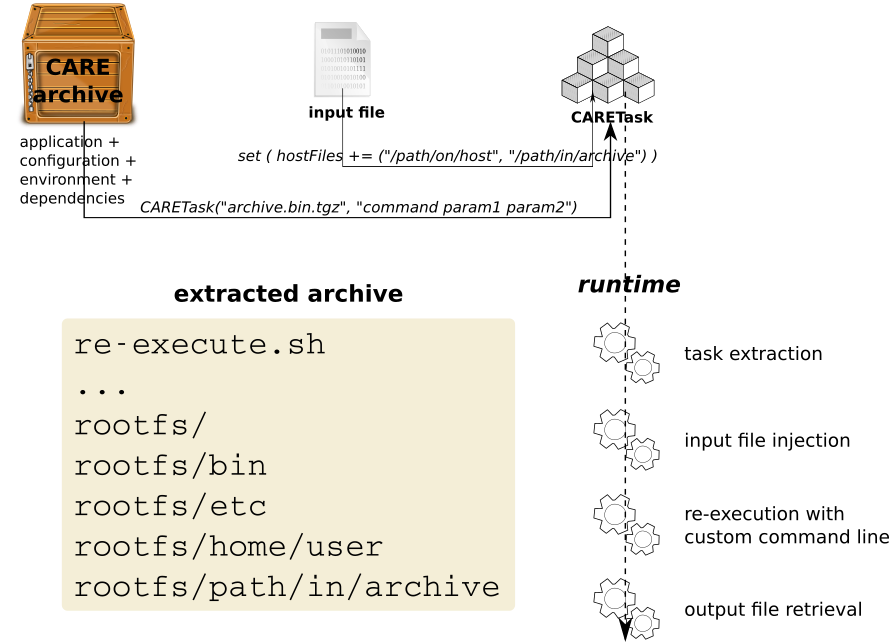
\includegraphics[width=0.8\linewidth]{OpenMOLECARE.png}
	\caption{Delegation of a task to remote execution environment in OpenMOLE. \cite{Leclaire2016}.}
	\label{OpenMOLECARE}
\end{figure}

\begin{listing}[h]
	\centering
	\begin{minipage}{13cm}
		\begin{minted}[frame=single,framesep=2mm,baselinestretch=1.15,fontsize=\small,linenos]{scala}
val output = Val[String]
val error = Val[String]
val value = Val[Int]

val pythonTask = 
  CARETask("hello.tgz.bin", "python hello.py /data/fileA.txt") set ( 
    stdOut := output,
    stdErr := error, 
    returnValue := value, 
    hostFiles += ("/home/user/fileA.txt", "/data/fileA.txt") 
  )
		\end{minted}
	\end{minipage}
	\caption{Example Python CARETask \cite{Leclaire2016}.}
	\label{CARETask}
\end{listing}

\subsection{Job Management}

Most of the logic of coordinating the execution of jobs and collection of results is handled by a \verb|JobManager| class. It uses a message queue to direct commands to separate actors responsible for uploading resources to execution nodes, submitting, querying or purging jobs, as in Listing \ref{JobManager}. 

The message queue is consumed iteratively by a unique dispatcher actor that routes messages to the specialised receiver actors. This model ensures a clear separation between individual actions carried out to monitor the jobs.

\begin{listing}[h]
	\centering
	\begin{minipage}{13.8cm}
		\begin{minted}[frame=single,framesep=2mm,escapeinside=||,baselinestretch=1,fontsize=\footnotesize,linenos]{scala}
class JobManager {
  ...
  def !(msg: JobMessage): Unit = msg match {
    case msg: Upload             |$\Rightarrow$| messageQueue.enqueue(msg)
    case msg: Submit             |$\Rightarrow$| messageQueue.enqueue(msg)
    case msg: Refresh            |$\Rightarrow$| messageQueue.enqueue(msg)
    case msg: GetResult          |$\Rightarrow$| messageQueue.enqueue(msg)
    case msg: KillBatchJob       |$\Rightarrow$| messageQueue.enqueue(msg)
    case msg: DeleteFile         |$\Rightarrow$| messageQueue.enqueue(msg)
    case msg: CleanSerializedJob |$\Rightarrow$| messageQueue.enqueue(msg)
    
    case Manage(job) |$\Rightarrow$|
      self ! Upload(job)
      
    case Delay(msg, delay) |$\Rightarrow$|
      delayedExecutor.schedule(self ! msg, delay.toMillis, TimeUnit.MILLISECONDS)
      
    case Uploaded(job, sj) |$\Rightarrow$|
      job.serializedJob = Some(sj)
      self ! Submit(job, sj)
      
    case Submitted(job, sj, bj) |$\Rightarrow$|
      val interval = job.environment.minUpdateInterval
      job.batchJob = Some(bj)
      self ! Delay(Refresh(job, sj, bj, interval), interval)
      
    case Kill(job) |$\Rightarrow$|
      job.state = ExecutionState.KILLED
      killAndClean(job)
      
    case Resubmit(job, storage) |$\Rightarrow$|
      killAndClean(job)
      job.state = ExecutionState.READY
      messageQueue.enqueue(Upload(job))      
    ...
}
		\end{minted}
	\end{minipage}
	\caption{Job lifecycle management.}
	\label{JobManager}
\end{listing}

\subsection{Environments}

Remote execution environments are added through a plugin system by implementing the \verb|BatchEnvironment| trait. This comes with a built-in \verb|JobManager| and various other defaults useful for modelling a generic job submission environment. \verb|ClusterEnvironment| is wrapper that ensures steady traffic flow to a cluster by limiting the number of outgoing connections and adds an interface for accessing storage via SSH.

Each concrete environment in OpenMOLE has a corresponding job service. The low-level mechanics of interacting with the scheduler and running individual jobs remotely are abstracted away in GridScale, so job services attached to environments decorate this behaviour with batch submission capabilities. 

\begin{listing}[h]
	\centering
	\begin{minipage}{14.2cm}
		\begin{minted}[frame=single,framesep=2mm,escapeinside=||,baselinestretch=1.15,fontsize=\small,linenos]{scala}
trait SGEJobService 
    extends ClusterJobService with SSHHost with SharedStorage { self |$\Rightarrow$|

  def environment: SGEEnvironment
  val jobService = new GridScaleSGEJobService with SSHConnectionCache {...}

  protected def _submit(serializedJob: SerializedJob) = {
    val (remoteScript, result) = buildScript(serializedJob)
    val jobDescription = new SGEJobDescription {
      val executable = "/bin/bash"
      val arguments = remoteScript
      val workDirectory = serializedJob.path
      override val queue = environment.queue
      override val wallTime = environment.wallTime
      override val memory = Some(environment.requiredMemory)
    }
    val jobId = self.jobService.submit(jobDescription)
    ...
  }
}
		\end{minted}
	\end{minipage}
	\caption{Job service used to submit batch jobs to the SGE scheduler.}
	\label{SGEJobService}
\end{listing}

Listing \ref{SGEJobService} shows the core of the \verb|SGEJobService|. Note that objects used to manage individual jobs on the underlying GridScale level are also called job services, so we must always consider the distinction. On line 8, a shell script embedding the task to be run is created from a serialized job. On line 11, the script is assigned to be run by \verb|bash| as part of an \verb|SGEJobDescription|. The job is then submitted to the underlying GridScale job service on line 17.

\section{GridScale} \label{GridScaleSection}

GridScale is the library part of the OpenMOLE ecosystem that mediates the access to distributed computing environments. Being written in Scala, it can be used as part of any application running on the Java Virtual Machine and it is designed around the strict type system of the Scala programming language. This leads to improved safety checks for job definitions at compile time, since their members can now be more refined than plain strings \cite{Reuillon2016}.

\subsection{Principles}

Historically, the scientific community has relied on specifications developed by the OGF\footnote{Open Grid Forum} \cite{OGF} to establish the guidelines for libraries used to access grids or clusters. However, a problem that standards like DRMAA\footnote{Distributed Resource Management Application API} \cite{DRMAA} or SAGA\footnote{Simple API for Grid Applications} \cite{SAGA} encounter is that they require the commitment of multiple parties interacting with an environment. Users need to implement a particular protocol that matches the version of the specification deployed by the administrators of the infrastructure. Additionally, the API is often slow to evolve and inflexible to user requirements.

GridScale chooses to stay away from particular standards and favours an approach where very few assumptions are made about the configuration of the target infrastructure. In particular, it only requires that the accessed environment runs a Linux distribution and the user has access to the \textit{bash} shell via SSH. This is reasonable to expect from most machines, since \textit{bash} is the default in most cases and a login shell is not needed. 

Jobs are submitted and monitored using the standard command line tools that would be manually invoked by the user. For example, SGE jobs are managed using \verb|qsub|, \verb|qstat| and \verb|qdel|, while SLURM jobs are managed using \verb|sbatch|, \verb|scontrol| and \verb|scancel| for submission, state querying and termination, respectively.

\subsection{Module Design}

Each environment accessed by GridScale is serviced by its own module in the implementation. Modules are packaged as independent OSGi\footnote{Open Service Gateway Initiative} \cite{OSGi} bundles so that they can be included individually by applications servicing only a specific infrastructure. This enforces a modular design and reduces the footprint of the library \cite{Reuillon2016}.

Every module corresponding to an environment consists of four different components wired together into a unique block using the cake pattern \cite{Cake}:

\begin{itemize}
	\item A \textit{Job Description} used to define the executable, arguments and other parameters for the job.
	\item A \textit{Job Service} responsible for the job submission mechanisms and resource acquisition.
	\item A \textit{Storage} component that can be shared across modules.
	\item An \textit{Authentication} rule for granting access rights using a login and password combination, SSH or certificate authentication.
\end{itemize}

Figure \ref{GridScaleArch} illustrates the creation of a SLURM module from particular implementations of the four component interface. Although the underlying technique in the cake pattern is different, it achieves a similar result to standard dependency injection in languages like Java by offering modules easy to assemble.

\begin{figure}[h]
	\centering
		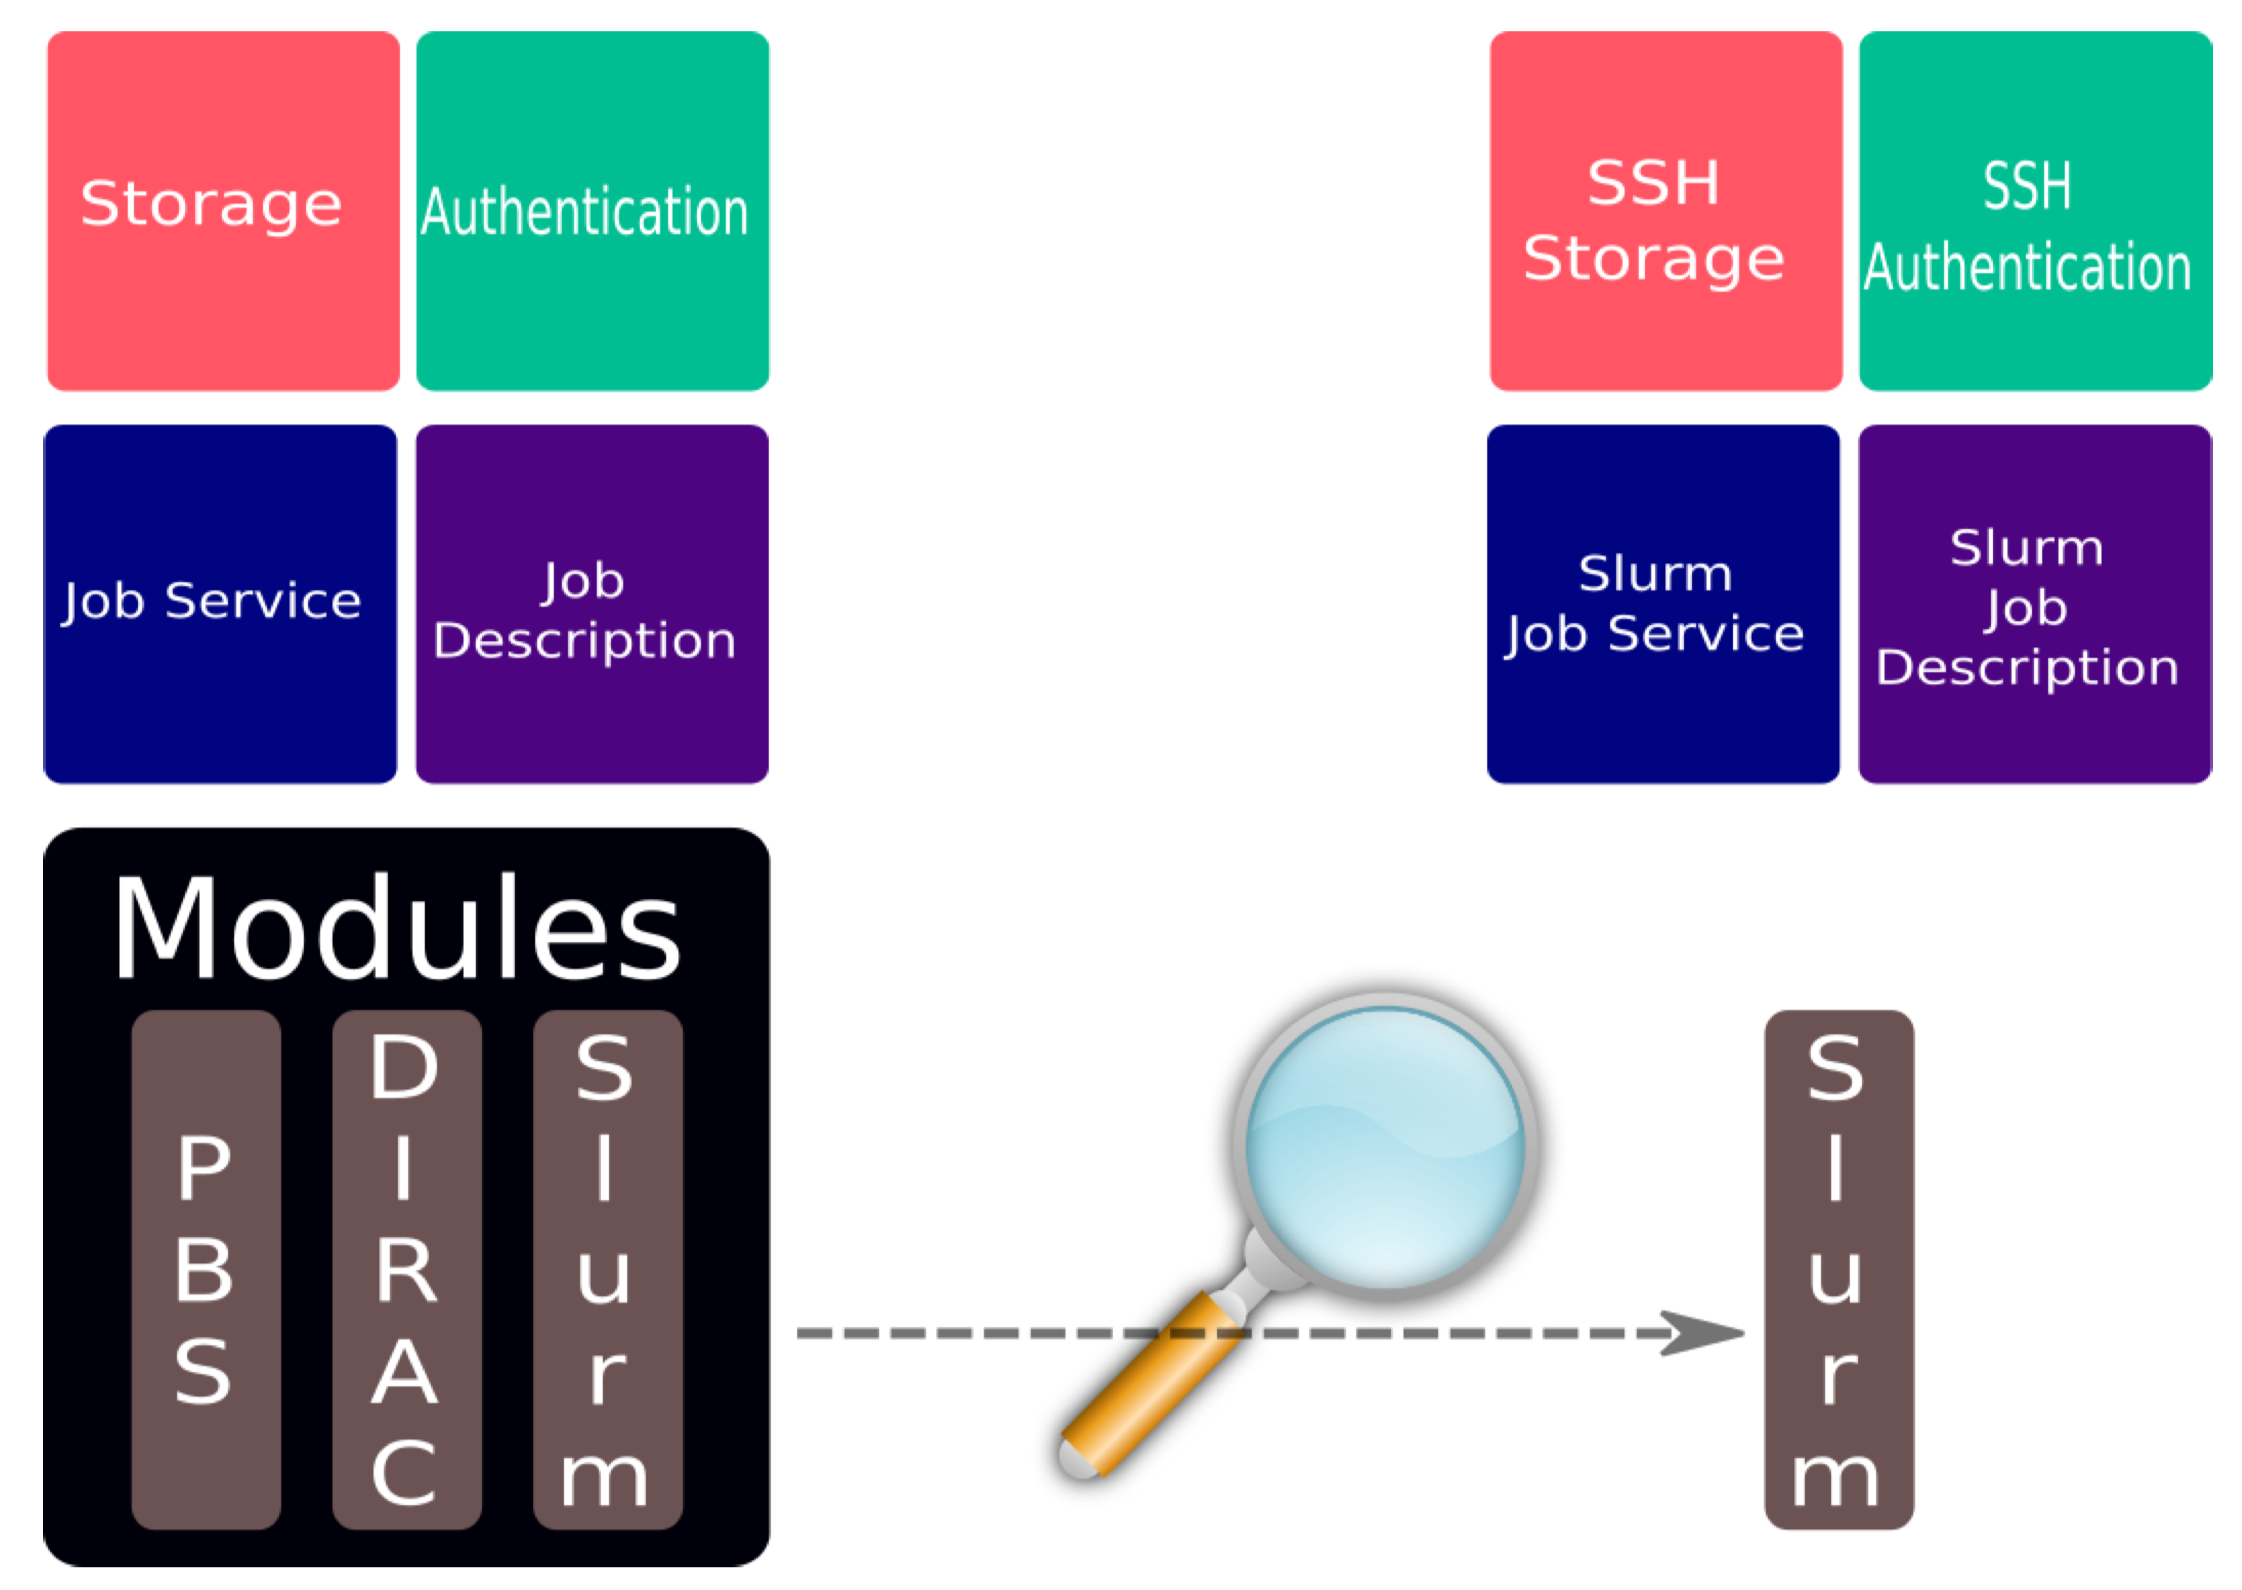
\includegraphics[width=0.65\linewidth]{GridScaleArch.png}
	\caption{GridScale architecture and instantiating the SLURM module \cite{Reuillon2016}.}
	\label{GridScaleArch}
\end{figure}

\vspace{4mm}
\textbf{Job Description}
\vspace{1mm}

Job descriptions are typesafe wrappers in Scala that translate to the plaintext scripts accepted by schedulers to queue jobs. The main advantage is that this ensures syntactical correctness of jobs and errors that would prevent jobs from being submitted are caught early. Silent issues such as misusing measurement unit for time or resources are also avoided by relying on a strong type system. 

Listing \ref{SLURMJobDescription} compares the definition of a simple SLURM job using the standard approach in a text \verb|bash| script and its equivalent counterpart in GridScale. Note that, even for a relatively short description, the plaintext version can easily become ambiguous in sections where durations or paths are specified.

\begin{listing}[h]
	\centering
	\begin{minipage}[b]{5.03cm}
		\begin{minted}[frame=single,framesep=2mm,escapeinside=||,baselinestretch=1.15,fontsize=\small]{text}
#!/bin/bash
#SBATCH -o job.out
#SBATCH -e job.err
#SBATCH --cpus-per-task=1 
#SBATCH --time=01:00:00
#SBATCH -D /home/foo/bar

/bin/echo success
        \end{minted}
	\end{minipage}
	\hspace{0.5cm}
    \begin{minipage}[b]{8.29cm}
		\begin{minted}[frame=single,framesep=2mm,escapeinside=||,baselinestretch=1.15,fontsize=\small]{scala}
val description = new SLURMJobDescription { 
  def executable = "/bin/echo"
  def arguments = "success"
  def workDirectory = "/home/foo/bar"
  override def wallTime = 1 hour
}
		\end{minted}
	\end{minipage}
	\caption{Comparison of a plaintext and a Scala SLURM job description.}
	\label{SLURMJobDescription}
\end{listing}

\vspace{3mm}
\textbf{Job Service}
\vspace{1mm}

The job service is the component that manages the lifecycle of jobs. Listing \ref{SLURMJobService} shows the creation of a job service capable of interacting with SLURM. To connect to the remote environment, the service relies on the presence of a target host and login, along with a possibly password-protected SSH private key.

\begin{listing}[h]
	\centering
	\begin{minipage}{14cm}
		\begin{minted}[frame=single,framesep=2mm,escapeinside=||,baselinestretch=1.15,fontsize=\small,linenos]{scala}
val slurmService = new SLURMJobService with SSHPrivateKeyAuthentication {
  def host = "host"
  def user = "user"
  def password = "password"
  def privateKey = new File("/path/to/private/key")
}
		\end{minted}
	\end{minipage}
	\caption{Job service used to submit batch jobs to the SLURM scheduler.}
	\label{SLURMJobService}
\end{listing}

The interface exposed by a job service consists of four main methods: \verb|submit|, \verb|state|, \verb|cancel| and \verb|purge|. These allow initiating jobs, checking their status, terminating them and cleaning up temporary data. 

In contract with other libraries used for distributed resource management libraries that retain caches of the system status, GridScale job services promote a functional approach and are designed to be immutable and hold as little state as possible. Therefore, all the public methods are pure and simply forward the request to the remote scheduler.

\vspace{3mm}
\textbf{Storage}
\vspace{1mm}

Storage wrappers abstract operations with files on the target environment. They are used by job services to set up the runtime by uploading files to remote machines and download results when jobs are done.

Standard POSIX file operations are also enabled in order to complement the usage of command line tools to delegate work. The implementation of all the connections and commands relies on the SSHJ \cite{SSHJ} library, which handles SSH connections and provides the SFTP\footnote{Secure File Transfer Protocol} primitives directly to Java or Scala.

\vspace{3mm}
\textbf{Authentication}
\vspace{1mm}

The authentication component provides access to all environments covered by GridScale. Private clusters are managed by opening an SSH connection to the master node, so the authentication consists of the address of this machine, the name of the user and a password or private key.

On the other hand, grids often require authentication methods that cover the security model of the middleware managing them. This is achieved in GridScale by allowing the installation of P12\footnote{PKCS - Public-Key Cryptography Standards} and PEM\footnote{Privacy Enhanced Mail} certificates \cite{Reuillon2016}.